

\section{\MethodnameLong}
\label{sec:method}
To alleviate the negative effects of data imbalance, we propose a comprehensive approach, \MethodnameLong{} (\Methodname), which aims to generate synthetic samples for minority classes. We first find the informative region where informative samples are located and balance this region by creating synthetic surrounding neighbors for minority samples. The remaining region is then fully balanced by arbitrarily generating minority samples' neighbors. We elaborate on how our strategy is developed in the rest of this section.

\subsection{Methodology Motivation}  

As Chazal and Michel mentioned in their work \cite{leroueil_compressibility_1996}, the natural way to highlight the global topological structure of the data is to connect data points' neighbors; our proposed method preserves their observation but in the reverse procedure, generating surrounding synthetic neighbors for minority samples. Thus, our method not only generates more data for minority class but also preserve the underlying topological structure of the entire data. 

Agreeing with the mutual idea in \cite{ertekin_learning_2007} and \cite{aggarwal_active_2020}, we believe that informative samples play the most important role in the prediction success of both traditional machine learning models (e.g., SVM, Naive Bayes) and modern deep learning approaches (e.g., neural network). Thus, our method finds these informative samples and focuses on augmenting minority data in this region. In this work, we apply an entropy-based active learning strategy mentioned in \ref{sec:EAL} to find the samples that maximize entropy to the model. This strategy is perhaps the most popular active learning technique and over-performs many other techniques on several datasets \cite{DAL}, \cite{7393573} \cite{settles_analysis_2008}.

\subsection{Generating minority synthetic data}  
%%This is how we generate synthetic data to maximize the fractional posterior:
A synthetic neighbor $ x'$ and its label $y'$ can be created surrounding a minority sample $x$ by adding a small random vector $v$ to the sample, $x' = x + v$. This lays on the d-sphere surface centered by $x$, and the d-sphere's radius is set by the length of vector $\vec{v}$, $|\vec{v}|$. It is, however, critical to generate synthetic data in the informative region because synthetic samples can unexpectedly jump across the decision boundary. This can be harmful to the model as this might create outliers and reduce the model's performance. Therefore, we safely find vector $\vec{v}$ towards the minority class such as $\vec{v}_0$ and $\vec{v}_1$ depicted in Figure \ref{fig:problem}. Our technique is described via a binary classification scenario as follows. 

Let consider a binary classification problem between majority class A and minority class B. 
From the Bayes' theorem, the posterior probabilities $p(y'=A|x')$ or $p(y'=B|x')$ can be used to present the probabilities that a synthetic sample $x'$ belongs to class A or class B, respectively. Let the two posterior probabilities be $f_0$ and $f_1$; they can be expressed as follows. 
\begin{align}
	\label{eq:posterior}
	p(y'=A|x') = \frac{p(x'|y'=A)\:p(A)}{p(x')} = f_0 \\
	p(y'=B|x') = \frac{p(x'|y'=B)\:p(B)}{p(x')} = f_1  
\end{align}

As mentioned earlier, we would like to generate each synthetic data $x'$ that maximizes the probability of $x'$ belonging to the minority class $B$ and minimizes the chance $x'$ falling into the majority class $A$. Thus, we propose a method that maximizes the fractional posterior $f$,   
\begin{align}
	\label{eq:fracpost}
	f &= f_1/f_0  \\
	&=\frac{p(x'|y'=B) \:p(B)}{p(x'|y'=A) \: p(A)}. \label{equ:f_ratio}
\end{align}


\textbf{\textit{Approximation of likelihoods in Equation \ref{equ:f_ratio}:}} We use non-parametric kernel density estimates (KDE) to approximate the likelihoods $p(x'|y'=A)$ and $p(x'|y'=B)$ as KDE is flexible and does not require specific assumptions about the data distribution. One can use a parametric statistical model such as Gaussian to approximate the likelihood; however, it oversimplifies the data and does not work effectively with topological complex data, especially in high dimensions. In addition, parametric models require an assumption about the distribution of data which is difficult in real-world problems since we usually do not have such information. On the other hand, KDE only needs a kernel working as a window sliding through the data. Among different commonly used kernels for KDE, we choose Gaussian Kernel as it is a powerful continuous kernel that would also eases the derivative computations for finding optima. 

\textbf{\textit{Approximation of priors in Equation \ref{equ:f_ratio}:}} Additionally, we assume prior probabilities of observing samples in class A ($p(A)$) and class B ($p(B)$) (in Equation \ref{equ:f_ratio}) are constant. Hence, these probabilities do not affect our algorithm in terms of generating synthetic neighbors for minority samples because we only determine the relative direction between the minority and the majority class. Thus, they can be canceled out at the end of the equation reduction. 

\textbf{\textit{Equation \ref{equ:f_ratio} reduction:} } Let $X_A$ and $X_B$ be the subsets of dataset $X$ which contain samples of class A and class B, $X_A=\{x: y=A  \}$ and $X_B=\{x: y=B  \}$. $N_A$ and $N_B$ are the numbers of samples in $X_A$ and $X_B$. $d$ is the number of data dimensions. $h$ presents the width parameter of the Gaussian kernel. The posterior ratio for each synthetic sample $x'$ then can be estimated as follows:

\begin{align}
	\label{eq:fracpost_estimation}
	f &= \frac{p(x'|y'=B)  \: p(B)}{p(x'|y'=A) \: p(A)} \\
	&\propto \frac{ \frac{1}{N_B h^d} \: \sum_{i=1}^{N_B}{ (2\pi)^{-\frac{d}{2}} \: e^{\frac{1}{2}{(\frac{x'-X_{B_i}}{h})^2} } } \: p(B) }
	{ \frac{1}{N_A h^d} \:  \sum_{j=1}^{N_A}{ (2\pi)^{-\frac{d}{2}} \: e^{ \frac{1}{2} {(\frac{x-X_{A_j}}{h})^2} } }\: p(A) }\\
	&\propto \frac{N_A}{N_B} \: \frac{ \sum_{i=1}^{N_B}{ e^{\frac{1}{2}{(\frac{x'-X_{B_i}}{h})^2} } } \: p(B)}
	{  \sum_{j=1}^{N_A}{ e^{ \frac{1}{2} {(\frac{x'-X_{A_j}}{h})^2} } } \: p(A)} \label{equ:f_}\\
	&\propto  \: \frac{ \sum_{i=1}^{N_B}{ e^{\frac{1}{2}{(\frac{x'-X_{B_i}}{h})^2} } }}
	{  \sum_{j=1}^{N_A}{ e^{ \frac{1}{2} {(\frac{x'-X_{A_j}}{h})^2} } } } \label{equ:f}.
\end{align} 


\textbf{\textit{Finding synthetic samples surrounding a minority sample:}} Because we want to generate neighbors for each minority sample that maximizes Function \text{f} in Equation \ref{equ:f}, we examine points lying on the sphere centered at the minority sample with a small radius $r$. As a result, we can find a vector $\vec{v}$ so that it can be added to the sample to generate a new sample. The relationship between a synthetic sample $x'$ and a minority sample can be described as follows,
\begin{align}
	\label{equ:vecV}
	\vec{x'} =  \vec{x} + \vec{v},
\end{align}
where $|\vec{v}| = r $, and $r$ is sampled from a uniform distribution $r \sim U(0,R)$, $0<r<R$. The range parameter $R$ is relatively small and computed as the average distance of k-nearest neighbors of the minority sample $x$ to itself. This will ensure that the generated sample will be surrounding the minority sample. Consider a minority sample $x$ and its k-nearest neighbors in the Euclidean space, $R$ can be computed as follows:

\begin{align}
	R = \frac{1}{k}\sum\limits_{1}^{k} ||x-x_j ||,
\end{align}
where $||x-x_j||$ is the Euclidean distance between a minority sample $x$ and its $j$th neighbor. $k$ is a parameter indicating number of the neighbors. In practice, we prefer to tune $k$ from 5 to 20.  


\begin{figure}[th!]
	%[trim=left bottom right top, clip]
	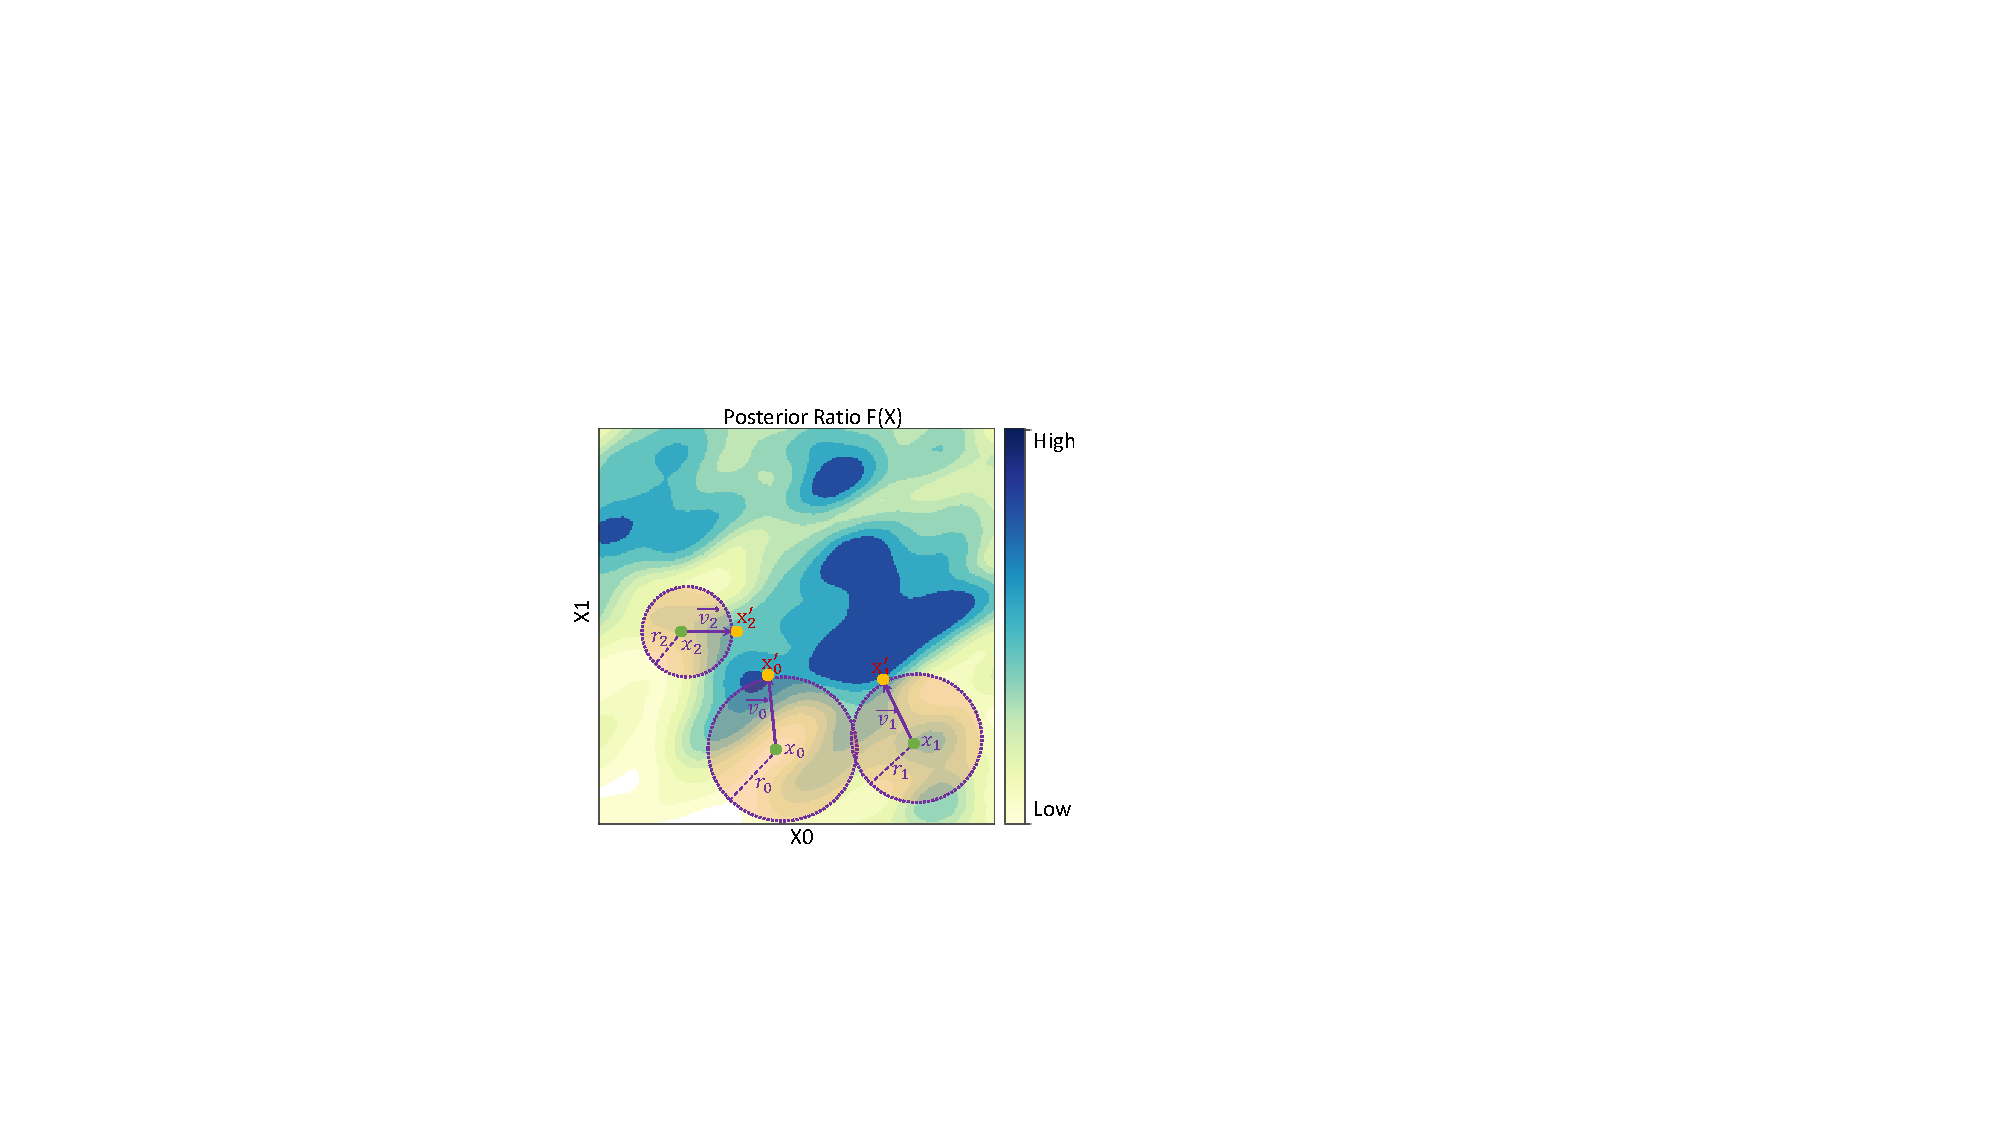
\includegraphics[width=\linewidth, trim=240 140 390 160,clip]{Figures/MaxPosteriorRatio/sphere_maxF.pdf}
	\caption{Demonstration on how \Methodname{} generates three synthetic samples $x'_0, x'_1, x'_2$, from three minority samples $x_0, x_1, x_2$, by maximizing the Posterior Ratio. }
	\label{fig:sphere_maxF}
\end{figure}

Figure \ref{fig:sphere_maxF} depicts a demonstration of finding 3 synthetic samples from 3 minority samples. In fact, one minority can be re-sampled to generate more than one synthetic sample. For a minority sample $x_0$, we find a synthetic sample $x_0'$ by maximizing the objective function $f(x_0'), x_0' \in X$ with a constraint that the Euclidean length of $\vec{v_0}$ equals to a radius $r_0$, $||\vec{v_0}|| = r_0$ or $||\vec{x_0'}-\vec{x_0}||=r_0$ (derived from Equation \ref{equ:vecV}). 


The problem can be described as a constrained optimization problem. For each minority sample $x$, we find a synthetic sample $x'\in \mathbb{R}^d$ lying on the d-sphere centered at $x$ with radius $r$ and maximizing function in Equation \ref{equ:f},
\begin{align}
	\label{prob:optimazation}
	\max_{x'} {f(x')} \;\;\; \textrm{s.t.}\; ||\vec{x'} - \vec{x}||=r,
\end{align}
where $r \sim U(0,R)$.

\textbf{\textit{Solving optimization problem in Equation \ref{prob:optimazation}:}} Interestingly, the problem in Equation\ref{prob:optimazation} is solvable. Function $f(x)$ in Equation \ref{equ:f} is defined and continuous for $x' \in (-\infty, +\infty)$ because all of the exponential components (Gaussian kernels) are continuous and greater than zero. In addition, the constraint, $||\vec{x'} - \vec{x}||=r$, which contains all points on the sphere centered at $x$ with radius $r$ is a closed set (\cite{wikipedia_2021}). Thus, a maximum exits as proved in \cite{maximum_exist}. To enhance the diversity of synthetic data, we accept either the global maximum or any local maximum, so that the synthetic samples will not simply go the same direction.  


We solve the problem in Equation \ref{prob:optimazation} by using the Projected Gradient Ascent approach in which we iteratively update the parameter to go up the gradient of the objective function. A local maximum is found if the objective value cannot be increased by any local update. For simplification, we rewrite the problem in Equation \ref{prob:optimazation} by shifting the origin to the considered minority sample. The problem becomes finding the maximum of function $f(x')$, $x' \in \mathbb{R}^d$, constrained on a d-sphere, i.e., $||x'||=r$. Our solution can be described in Algorithm \ref{alg:optimization}. After shifting the coordinates system, we start with sampling a random point on the constraint sphere (line $1-2$). The gradient of objective function at time $t$, $g_t(x'_t)$, is computed and projected onto sphere tangent plane as $p_t$ (line $4-5$). It is then normalized and used for update a new $x'_{t+1}$ by rotating a small angle $lr*\theta$ (line $6-7$). The algorithm stops when the value of $f(x')$ is not increased by any update of $x'$. We finally shift to the original coordinates and return the latest $x'_t$.   

\begin{algorithm}[h]
	\caption{Sphere-Constrained Gradient Ascent for Finding Maximum}
	
	\begin{flushleft}
		\textbf{Input}: A minority sample $x_0$, objective function $f(x,X)$\\
		\textbf{Parameter}: \\
		$r$ : The radius of the sphere centered at $x_0$  \\\
		$\theta$ : Sample space $\theta \in [0,2\pi]$ \\
		$lr$ : Gradient ascent learning rate\\
		
		\textbf{Output}: An local maximum $x'$\\
		\begin{algorithmic}[1]
			\STATE Shift the Origin to $x_0$
			\STATE Randomly initiate $x'_t$ on the sphere with radius $r$	
			\WHILE {converge condition}
			\STATE Compute the gradient at $x'_t$\\
			$g_t(x'_t) = \nabla f(x'_t)$
			\STATE Project the gradient onto the sphere tangent plane\\
			$p_t = g_t - (g_t \cdot x'_t) x_t$
			\STATE Normalize projected vector\\
			$p_t = p_t/ ||p_t||$
			\STATE Update $x'$ on the constrained sphere \\
			$x'_{t+1} = x'_t cos(lr*\theta) + p_t sin (lr*\theta)$ 			
			\ENDWHILE
			\STATE Shift back to the Origin
			\RETURN $x'_t$
		\end{algorithmic}
	\end{flushleft}
	\label{alg:optimization}
\end{algorithm}

\subsection{Algorithm}
Our strategy can be described in Algorithm \ref{alg:SIMPOR}. Our algorithm takes an imbalanced dataset as its input and results in a balanced dataset which is a combination of the original dataset and synthetic samples. We first choose an active learning method $AL(\cdot)$ and find a subset of informative samples $S$, which is shown in lines $1-2$ in Algorithm \ref{alg:SIMPOR}. In this work, we choose entropy-based active learning for our experiments. We then generate synthetic data to balance $S$. For each random sample $x_i^c$ in $S$ and belonging to minority class $c$, we randomly sample a small radius $r$ and find a synthetic sample that lies on the sphere centered at $x_i^c$ and maximizes the posterior ratio in Equation \ref{equ:f} (lines $3-11$). The process is repeated until the informative set $S$ is balanced. Similarly, the remaining region is balanced which can be described in the pseudo-code from line $12$ to line $20$. The final output of the algorithms is a balanced dataset $D'$.       

\begin{algorithm}[!htb]
	\caption{\Methodname}
	
	\begin{flushleft}
		\textbf{Input}: Original Imbalance Dataset $D$ including data $X$ and labels $y$.\\
		\textbf{Parameter}: 
		$MA$ is the majority class, $MI$ is a set of other classes.\\
		$k$: Number of  neighbors of the considered sample which determines the maximum range of the sample to its synthetic samples.\\ 
		$Count(c, P)$ : A function to count class $c$ sample number in population $P$.\\
		$G(x_0,f,r)$ : Algorithm \ref{alg:optimization}, which returns a synthetic sample on sphere centered at $x_0$ with radius $r$ and maximize Equation \ref{equ:f}.  \\
		\textbf{Output}: Balanced Dataset $D'$ including $\{X',y'\}$
		\begin{algorithmic}[1]
			\STATE Select an Active Learning Algorithm $AL()$
			\STATE Query a subset of informative samples $S \in D$  using $AL$:
			$s  \leftarrow AL(D) $	\\
			
			\COMMENT{Balance the informative region}
			\FOR {$c \in MI$}
			\WHILE {$Count(c, S) \leq Count(MA, S)$ }
			\STATE Select a random $x_i^c \in S$
			\STATE Compute maximum range $R$ based on $k$
			\STATE  Randomly sample a radius $r \sim U(0,R)$
			\STATE Generate a synthetic neighbor $x'$ from $x_i^c$:
			$x'=G(x_i^c,f,r)$ 
			\STATE Append $x'$ to $D'$
			\ENDWHILE
			\ENDFOR
			
			\COMMENT{Balance the remaining region}
			\FOR {$c$ in $MI$}
			\WHILE { $Count(c, D') \leq Count(MA, D')$ }	
			\STATE Select a random $x_j^c \in \{X-S\}$
			\STATE Compute maximum range $R$ based on $k$
			\STATE  Randomly sample a radius $r \sim U(0,R)$
			\STATE Generate a synthetic neighbor $x'$ of $x_j^c$ 
			\STATE Append $x'$ to $D'$
			\ENDWHILE
			\ENDFOR
			\RETURN 
		\end{algorithmic}
	\end{flushleft}
	\label{alg:SIMPOR}
\end{algorithm}